\problemname{Workers of the World Unite! Just Not Too Close.}

You are in charge of a set of workers working on a project so top secret we can't even think of a name for it.  They are each housed separately in a set of apartments shown on the left in figure \ref{fig:layout} and every morning they each leave at the same time and proceed to one of the workstations shown on the right.  In order to get from their homes to the workstations they must pass through a security gate shown in the middle.  Each gate has two different corridors that can be used, labeled A and B.  As can be seen from the figure the A corridors in each gate are always to the north of the B corridors.

\setlength{\unitlength}{3pt}
\begin{figure}[!h]
\centering
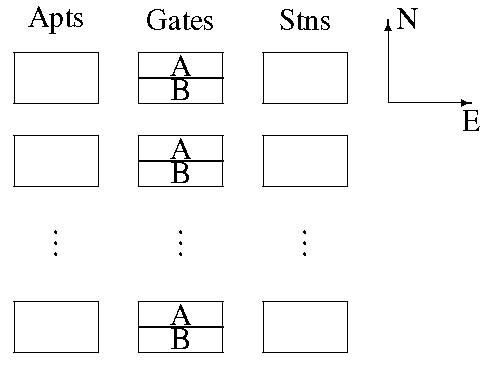
\includegraphics[width=0.5\textwidth]{workers_fig.png}
%\begin{picture}(55,45)(0,0)
%\put( 0, 0){\framebox(10,6){}}
%\put(15, 0){\framebox(10,3){B}}
%\put(15, 3){\framebox(10,3){A}}
%\put(30, 0){\framebox(10,6){}}
%\put( 5,14){\makebox(0,0){$\vdots$}}
%\put(20,14){\makebox(0,0){$\vdots$}}
%\put(35,14){\makebox(0,0){$\vdots$}}
%\put( 0,20){\framebox(10,6){}}
%\put(15,20){\framebox(10,3){B}}
%\put(15,23){\framebox(10,3){A}}
%\put(30,20){\framebox(10,6){}}
%\put( 0,30){\framebox(10,6){}}
%\put(15,30){\framebox(10,3){B}}
%\put(15,33){\framebox(10,3){A}}
%\put(30,30){\framebox(10,6){}}
%\put( 5,40){\makebox(0,0){Apts}}
%\put(20,40){\makebox(0,0){Gates}}
%\put(35,40){\makebox(0,0){Stns}}
%\put(45,30){\vector(0,1){10}}
%\put(45,30){\vector(1,0){10}}
%\put(46,40){\makebox(0,0)[l]{N}}
%\put(55,29){\makebox(0,0)[t]{E}}
%\end{picture}
\caption{Layout of apartments, gates and workstations.}
\label{fig:layout}
\end{figure}

Getting the workers to the workstations sounds simple, but with the onset of COVID-$19$ a problem has arisen.  First, because of social distancing no two workers can use the same gate.  Second, because of the layout of the gates, if one worker uses an A corridor, the person using the gate to the north of them cannot use the B corridor -- it's too close.  The analogous thing occurs if a worker uses a B corridor -- the worker using the gate to the south of them can't use the A corridor.

You are in charge of assigning workers to the stations, one worker at each station.  It doesn't matter which worker is assigned to which workstation but you would like to minimize the total distance all the workers travel while adhering to the social distancing requirements described above.  Due to the strange layout of the entrances and exits to the gates there can sometimes be large differences in distances when using the A corridor versus the B corridor for a gate, which complicates the problem.  Given all the relative distances, determine an assignment of workers to workstations that minimizes the total distance everyone travels.


\section*{Input}

Input begins with a line containing one positive integer $n \leq 50$, specifying the number of workers, gates and workstations, each numbered $1$ to $n$. Following this are $n$ lines each containing $2n$ positive integers.  The $i$-th of these lines gives the distance from worker $i$ to the entrances of the $n$ gates; the first two values are the distances to corridors A and B for gate $1$, the second two values are the distances to corridors A and B for gate $2$, and so on.  After this are $n$ more lines each containing $2n$ positive integers.  The $j$-th of these lines gives the distance from the workstation $j$ to the exits of the $n$ gates in an analogous fashion.  All distances are positive and $ \leq 1\; 000$.

\section*{Output}

On the first line of output print the minimum total distance traveled by the workers that can be achieved.  Follow this with $n$ lines showing the assignment for each worker.  The $i$-th of these lines will have the form $i$ $g_i$ $w_i$ indicating that worker $i$ uses gate $g_i$ to get to workstation $w_i$.  Use the format shown in the sample output. If there are several optimal assignments, any will be accepted
